\documentclass[11pt, a4paper]{book}

\usepackage{tikz,tikz-cd}
\usetikzlibrary{
    shapes,% for the rectangle
    chains,% provides the chains
    scopes,
    arrows,%
    matrix,%
    positioning,% wg. " of "
    scopes,%
    decorations.pathmorphing,% /pgf/decoration/random steps | erste Graphik
    shadows%
}% allows to replace \begin{scope} \end{scope} with {}


\begin{document}
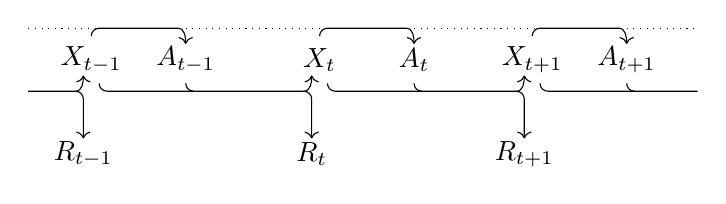
\begin{tikzpicture}
    \draw[dotted] (-3.7,0.4) -- (-2.8,0.4);

    \draw[->] (-3.7, -0.4) %%% transition stub beginning
    to [out=0,in=180] (-3.1, -0.4)
    to [out=0,in=270] (-3, -0.2);

    \draw[->] (-3.1, -0.4) %%% to R_{t-1}
    to [out=0,in=90] (-3,-0.5)
    to [out=270, in=90] (-3,-1);

    \draw (-3,-1.2) node {\(R_{t-1}\)};
    \draw (-2.9,0) node {\(X_{t-1}\)};

    \draw[->] (-2.9,0.3) %%% X_{t-1} to A_{t-1}
    to [out=90,in=180] (-2.8, 0.4) 
    to [out=0,in=180] (-1.8,0.4)
    to [out=0,in=90] (-1.7,0.2);

    \draw[dotted] (-1.7,0.4) -- (0.1,0.4);

    \draw (-1.7,0) node {\(A_{t-1}\)};

    \draw (-1.7, -0.3) %%% join transition 
    to [out=270,in=180] (-1.6,-0.4);

    \draw[->] (-2.8, -0.3) %%% X_{t-1} to X_t transition
    to [out=270,in=180] (-2.7, -0.4) 
    to [out=0,in=180] (-0.2, -0.4)
    to [out=0,in=270] (-0.1, -0.2);

    \draw[->] (-0.2, -0.4) %%% to R_t
    to [out=0,in=90] (-0.1,-0.5)
    to [out=270, in=90] (-0.1,-1);

    \draw (-0.1,-1.2) node {\(R_t\)};
    \draw (0,0) node {\(X_t\)};
    
    \draw[->] (0,0.3)  %%% X_t to A_t
    to [out=90,in=180] (0.1, 0.4) 
    to [out=0,in=180] (1.1,0.4)
    to [out=0,in=90] (1.2,0.2); 

    \draw[dotted] (1.2,0.4) -- (2.8,0.4);
 
    \draw (1.2,0) node {\(A_t\)};

    \draw (1.2, -0.3) %%% join transition
    to [out=270,in=180] (1.3,-0.4);

    \draw[->] (0.1, -0.3) %%% X_t to X_{t+1} transition
    to [out=270,in=180] (0.2, -0.4) 
    to [out=0,in=180] (2.5, -0.4)
    to [out=0,in=270] (2.6, -0.2);

    \draw[->] (2.5, -0.4) %%% to R_{t+1}
    to [out=0,in=90] (2.6,-0.5)
    to [out=270, in=90] (2.6,-1);

    \draw (2.6,-1.2) node {\(R_{t+1}\)};
    \draw (2.7,0) node {\(X_{t+1}\)};

    \draw[->] (2.7,0.3)  %%% X_{t+1} to A_{t+1}
    to [out=90,in=180] (2.8, 0.4) 
    to [out=0,in=180] (3.8,0.4)
    to [out=0,in=90] (3.9,0.2); 

    \draw[dotted] (3.9,0.4) -- (4.8,0.4);

    \draw (3.9,0) node {\(A_{t+1}\)};

    \draw (3.9, -0.3) %%% join transition stub
    to [out=270,in=180] (4,-0.4);

    \draw (2.8, -0.3) %%% X_{t+1} transition stub end
    to [out=270,in=180] (2.9, -0.4) 
    to [out=0,in=180] (4.8, -0.4);
\end{tikzpicture}
\end{document}

